% Draft target schematics only; no activity or scoring code.
% Adapted from the tikz-generation template and circuit-layout references.
\documentclass[tikz,border=4pt,multi=tikzpicture]{standalone}
\usepackage[siunitx,RPvoltages]{circuitikz}
\usepackage{fontspec}
\setmainfont{Linux Libertine O}
\usepackage{unicode-math}
\setmathfont{TeX Gyre Pagella Math}
\usepackage{xeCJK}
\setCJKmainfont{FangSong}
\definecolor{ink}{HTML}{17212E}
\tikzset{every picture/.style={draw=ink,text=ink,line width=0.85pt,
  font=\fontsize{15}{18}\selectfont},every node/.style={inner sep=3pt}}
\ctikzset{bipoles/length=1.4cm,bipoles/thickness=1.3,
  nodes width=0.055,bipoles/cuteswitch/thickness=0.25}
\begin{document}

% 01: one lamp, one switch and one cell in a single loop.
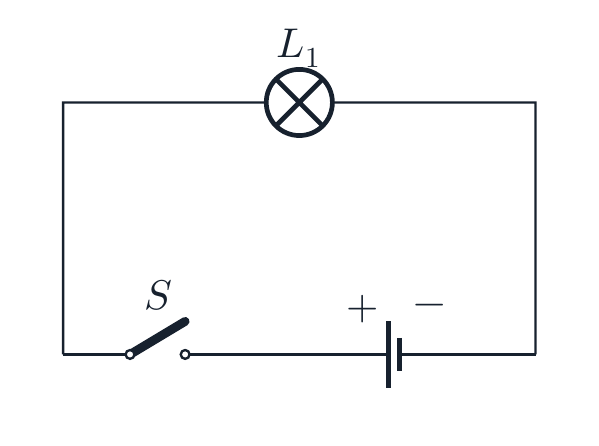
\begin{tikzpicture}[european]
  \path[use as bounding box] (-0.45,-0.8) rectangle (6.45,4.15);
  \draw (0,0) -- (0,3.2) to[lamp,l=$L_1$] (6,3.2) -- (6,0);
  \draw (0,0) to[cosw,l=$S$] (2.4,0)
    to[battery1,invert] (6,0);
  \node at (3.8,0.57) {$+$};
  \node at (4.65,0.57) {$-$};
\end{tikzpicture}

% 02: two lamps in series; the switch controls the entire loop.
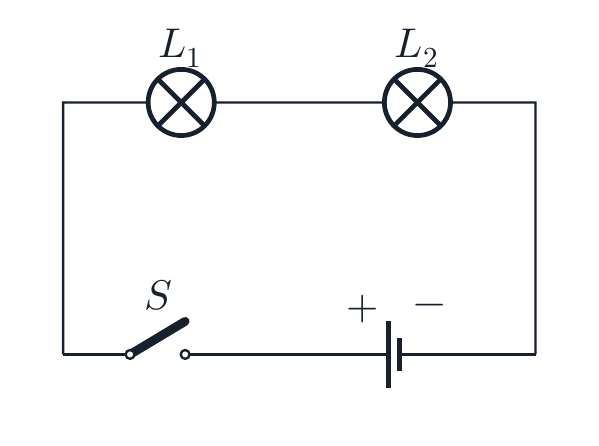
\begin{tikzpicture}[european]
  \path[use as bounding box] (-0.45,-0.8) rectangle (6.45,4.15);
  \draw (0,0) -- (0,3.2) to[lamp,l=$L_1$] (3,3.2)
    to[lamp,l=$L_2$] (6,3.2) -- (6,0);
  \draw (0,0) to[cosw,l=$S$] (2.4,0)
    to[battery1,invert] (6,0);
  \node at (3.8,0.57) {$+$};
  \node at (4.65,0.57) {$-$};
\end{tikzpicture}

% 03: two parallel lamps; S is outside both branches.
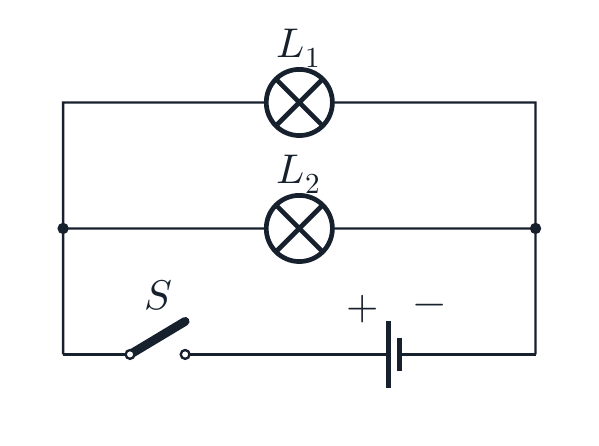
\begin{tikzpicture}[european]
  \path[use as bounding box] (-0.45,-0.8) rectangle (6.45,4.15);
  \draw (0,0) -- (0,3.2) to[lamp,l=$L_1$] (6,3.2) -- (6,0);
  \draw (0,1.6) to[lamp,l=$L_2$,*-*] (6,1.6);
  \draw (0,0) to[cosw,l=$S$] (2.4,0)
    to[battery1,invert] (6,0);
  \node at (3.8,0.57) {$+$};
  \node at (4.65,0.57) {$-$};
\end{tikzpicture}

% 04: S controls both branches; S1 controls L1 only.
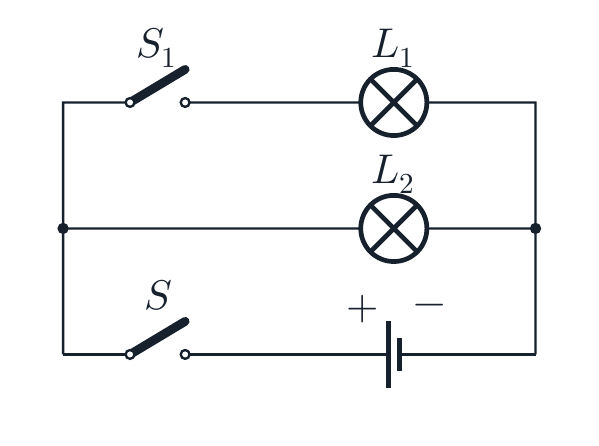
\begin{tikzpicture}[european]
  \path[use as bounding box] (-0.45,-0.8) rectangle (6.45,4.15);
  \draw (0,0) -- (0,3.2) to[cosw,l=$S_1$] (2.4,3.2)
    to[lamp,l=$L_1$] (6,3.2) -- (6,0);
  \draw (0,1.6) to[short,*-] (2.4,1.6)
    to[lamp,l=$L_2$,-*] (6,1.6);
  \draw (0,0) to[cosw,l=$S$] (2.4,0)
    to[battery1,invert] (6,0);
  \node at (3.8,0.57) {$+$};
  \node at (4.65,0.57) {$-$};
\end{tikzpicture}

% 05: (S1 + L1) in parallel with L2; that group is in series with L3.
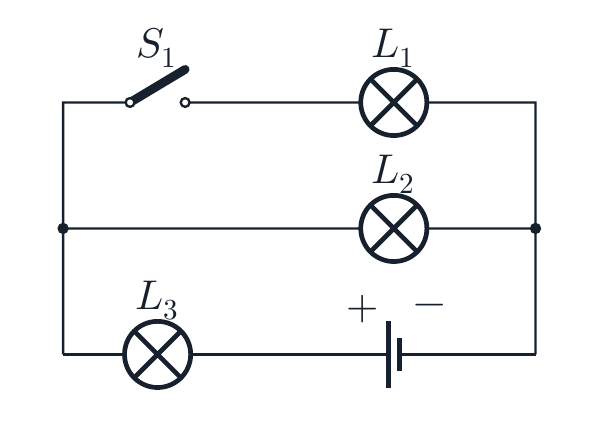
\begin{tikzpicture}[european]
  \path[use as bounding box] (-0.45,-0.8) rectangle (6.45,4.15);
  \draw (0,0) -- (0,3.2) to[cosw,l=$S_1$] (2.4,3.2)
    to[lamp,l=$L_1$] (6,3.2) -- (6,0);
  \draw (0,1.6) to[short,*-] (2.4,1.6)
    to[lamp,l=$L_2$,-*] (6,1.6);
  \draw (0,0) to[lamp,l=$L_3$] (2.4,0)
    to[battery1,invert] (6,0);
  \node at (3.8,0.57) {$+$};
  \node at (4.65,0.57) {$-$};
\end{tikzpicture}

\end{document}
